\documentclass[11pt, letterpaper, twocolumn, fleqn]{article}
\usepackage[margin=0.5in]{geometry}
\usepackage[utf8]{inputenc}
\usepackage{amsmath,amssymb,amsthm,graphicx}
\graphicspath{ {./images/} }

\let\oldemptyset\emptyset
\let\emptyset\varnothing

\begin{document}
    \renewcommand{\labelenumi}{\alph{enumi}.}
    \renewcommand{\labelenumii}{(\arabic{enumii})}
    \renewcommand{\qedsymbol}{$\blacksquare$}
    
    \paragraph{4.1.1}
        \begin{enumerate}
            \item 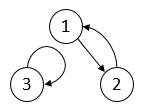
\includegraphics[scale=.7]{411a}
            \item 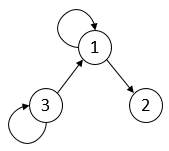
\includegraphics[scale=.7]{411b}
            \item 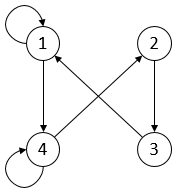
\includegraphics[scale=.7]{411d}
            \item 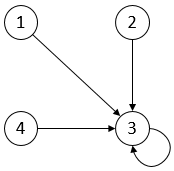
\includegraphics[scale=.7]{411f}
        \end{enumerate}
    
    \paragraph{4.1.2}    
        \begin{enumerate}
            \item 
                $\begin{bmatrix}
                    1 & 1 & 1 \\
                    0 & 0 & 0 \\
                    0 & 0 & 0
                \end{bmatrix}$
            \addtocounter{enumi}{3}
            \item 
                $\begin{bmatrix}
                    1 & 0 & 0 & 1 \\
                    0 & 1 & 0 & 0 \\
                    0 & 0 & 1 & 0 \\
                    1 & 0 & 0 & 1
                \end{bmatrix}$
            \item 
                $\begin{bmatrix}
                    1 & 0 & 0 & 1 \\
                    1 & 0 & 0 & 0 \\
                    0 & 1 & 1 & 0 \\
                    0 & 0 & 1 & 0 \\
                \end{bmatrix}$
        \end{enumerate}

    \paragraph{4.1.4}
        \begin{enumerate}
            \item 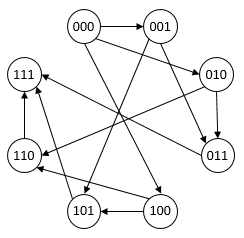
\includegraphics[scale=.7]{414a}
            \item 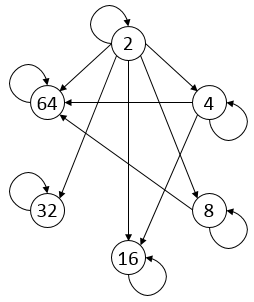
\includegraphics[scale=.7]{414b}
            \item 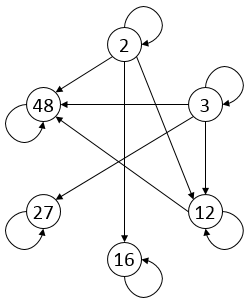
\includegraphics[scale=.7]{414c}
            \item 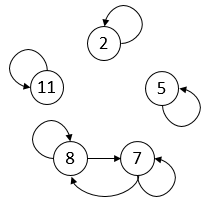
\includegraphics[scale=.7]{414d}
        \end{enumerate}
        
    \paragraph{4.2.1}
        \begin{enumerate}
            \item Anti-reflexive because $x < x$ is never true. 
                  Anti-symmetric because if $x < y$ then y cannot be less than x.
                  Transitive because if $x < y$ and $y < z$ then $x < z$
            \item Reflexive because $x \leq x$ is always true.
                  Anti-symmetric because if $x \neq y$ and $x \leq y$ then y cannot be less than x.
                  Transitive because if $x \leq y$ and $y \leq z$ then $x \leq z$
            \item Reflexive because $x^n = x$ when $n=1$.
                  The relation is anti-symmetric because the $x^n = y$ and $y^m = x$ are only true for some positive integer m and n when $x = y$ and $m=n=1$.
                  Transitive because if $x^n=y$ and $y^m=z$ for some positive integer n and m, then $z = (x^n)^m = x^{nm}$. 
            \item Reflexive because for any positive integer x, $x=x*1$ so xDx.
                  Anti-symmetric, x evenly divides y implies $x \leq y$. $y \leq x$ can only be true if $y=x$, therfore, the relation is anti-symmetric.
                  Transitive. xDy implies $y=xn$ for some positive integer n. yDz implies $z=ym$ for some positive integer m. Combining these gives $z=nmx$ which implies that xDz, therfore the relation is transitive.
            \item Reflexive. $|x-x| \leq 2$ becomes $0 \leq 2$ which is always true.
                  Symmetric because $|x-y| = |y-x|$
                  Not transitive because $|0-2| \leq 2$ and $|2-4| \leq 2$ but $|0-4| \nleq 2$
            \item Reflexive because $x-x=0$.
                  Symmetric because $x - y$ is rational and $y - x$ is rational.
                  Transitive because if $x-y$ is rational and $y-z$ rational then $x-z$ is rational.
        \end{enumerate}
    
    \paragraph{4.2.3}
        \begin{enumerate}
            \item No, a reflexive relation implies that for every $x \in R$, it is true that xRx. A anti-reflexive relation implies that for every $x \in R$, it is false that xRx.
            \item No a symmetric relation implies that for every $x \in R$ it is true that xRy and yRx. An anti-symmetric relation implies that for every $x \in R$ it is false that xRy and yRx.
        \end{enumerate}
    
    \paragraph{4.2.5}
        \begin{enumerate}
            \item 
                \begin{enumerate}
                    \item Anti-reflexive because $|A-A| = |\emptyset| = 0 \neq 1$ 
                    \item Neither symmetric nor anti-symmetric. Not symmetric because if $A=\{a,b\}$ and $B=\{b\}$ then $|A-B| = |\{a\}| = 1$ which does not equal $|B-A| = |\emptyset| = 0$. Not anti-symmetric because if $A=\{a,b\}$ and $B=\{b,c\}$ then $A \neq B$ and 
                        $$|A-B| = |\{a\}| = 1 = |\{b\}| = |B-A|$$
                    \item Not transitive. If A = \{a,c\}, B=\{a,b\}, and C=\{b\} then 
                    \begin{align*}
                        |A-B| &= |\{c\}| = 1 \\
                        |B-C| &= |\{a\}| = 1 \\
                        |A-C| &= |\{a,e\}| = 2
                    \end{align*}
                \end{enumerate}
            \item
                \begin{enumerate}
                    \item Anti-reflexive because $A \cap A = A \neq \emptyset$
                    \item Symmetric because $A \cap B = \emptyset = B \cap A$
                    \item Not transitive because if $A = \{a,b\}, B=\{c\}, C=\{a\}$ then $A \cap B = \emptyset$ and $B \cap C = \emptyset$ and $A \cap C = \{a\} \neq \emptyset$
                \end{enumerate}
        \end{enumerate}
    
    \paragraph{4.3.1}
        \begin{enumerate}
            \item 2
            \item 3
            \item c
            \item g
            \item There are no self loops in the graph.
            \item It is not a walk, trail, or path because there is no edge $(f,c)$.
        \end{enumerate}
    
    \paragraph{4.3.2}
        \begin{enumerate}
            \item It is a circuit, but not a cycle.
            \item $\langle d,b,c,g,f,d \rangle$ with a length of 5.
            \item $\langle c,g,f,e,c \rangle$
            \item $\langle d,b,c,g,f,d \rangle$
            \item $\langle d,b,c,f \rangle$
        \end{enumerate}
    
    \paragraph{4.5.1}
        \begin{enumerate}
            \item No
            \item Yes $\langle b,c,f,e \rangle$
            \item No
            \addtocounter{enumi}{1}
            \item Yes $\langle b,c,d,b \rangle$
        \end{enumerate}
    
    \paragraph{4.5.2}
        \begin{enumerate}
            \item 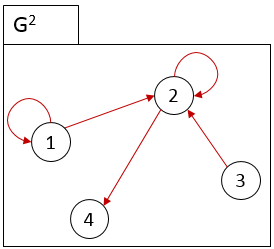
\includegraphics[scale=.7]{452a1} \newline
                  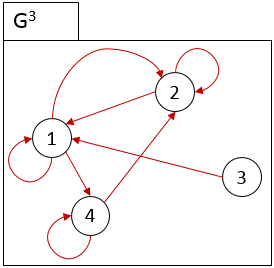
\includegraphics[scale=.7]{452a2} \newline
                  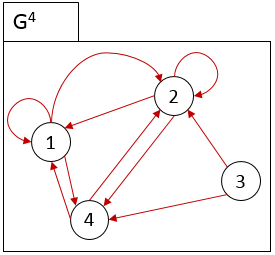
\includegraphics[scale=.7]{452a3} \newline
                  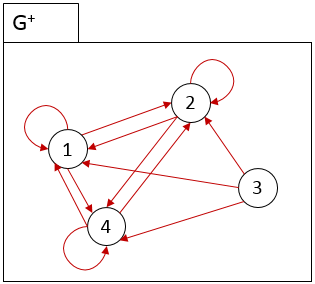
\includegraphics[scale=.7]{452a4} 
        \end{enumerate}
    
    \paragraph{4.5.3}
        \begin{enumerate}
            \item 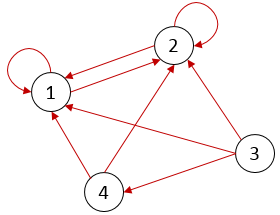
\includegraphics[scale=.7]{453a}
            \item 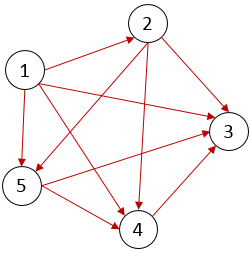
\includegraphics[scale=.7]{453b}
        \end{enumerate}
    
    \paragraph{4.6.1}
        \begin{enumerate}
            \item 
                \begin{align*}
                    A &=   \begin{bmatrix}
                            0 & 1 & 0 & 0\\
                            0 & 0 & 1 & 0\\
                            0 & 0 & 0 & 1\\
                            0 & 1 & 0 & 0
                           \end{bmatrix} \\                  
                    A^2 &= \begin{bmatrix}
                            0 & 0 & 1 & 0\\
                            0 & 0 & 0 & 1\\
                            0 & 1 & 0 & 0\\
                            0 & 0 & 1 & 0 
                           \end{bmatrix} \\
                    A^3 &= \begin{bmatrix}
                            0 & 0 & 0 & 1\\
                            0 & 1 & 0 & 0\\
                            0 & 0 & 1 & 0\\
                            0 & 0 & 0 & 1
                           \end{bmatrix} \\
                    A^4 &= \begin{bmatrix}
                            0 & 1 & 0 & 0\\
                            0 & 0 & 1 & 0\\
                            0 & 0 & 0 & 1\\
                            0 & 1 & 0 & 0
                           \end{bmatrix} \\
                    A^+ &= \begin{bmatrix}
                            0 & 1 & 1 & 1\\
                            0 & 1 & 1 & 1\\
                            0 & 1 & 1 & 1\\
                            0 & 1 & 1 & 1
                           \end{bmatrix}
                \end{align*}
        \end{enumerate}
    
    \paragraph{4.6.2}
        \begin{enumerate}
            \item 
                $$A =   \begin{bmatrix}
                        0 & 0 & 0 & 0 & 0 & 1\\
                        1 & 0 & 0 & 0 & 0 & 0\\
                        0 & 1 & 0 & 1 & 0 & 0\\
                        0 & 0 & 1 & 0 & 1 & 0\\
                        0 & 0 & 0 & 0 & 1 & 1\\
                        0 & 1 & 0 & 0 & 0 & 0
                        \end{bmatrix}$$
            \item
                $$A^2 = \begin{bmatrix}
                        0 & 1 & 0 & 0 & 0 & 0\\
                        0 & 0 & 0 & 0 & 0 & 1\\
                        1 & 0 & 1 & 0 & 1 & 0\\
                        0 & 1 & 0 & 1 & 1 & 1\\
                        0 & 1 & 0 & 0 & 1 & 1\\
                        1 & 0 & 0 & 0 & 0 & 0
                        \end{bmatrix}$$
            \item 2, 4, 5, and 6
        \end{enumerate}
    
    \paragraph{4.7.1}
        \begin{enumerate}
            \item J, I, B, A, F
            \item E, D
            \item (A,D),(G,F),(D,B),(H,I)
        \end{enumerate}
    
    \paragraph{4.8.1}
        \begin{enumerate}
            \item Not an equivalence relation because it is not transitive. If x shares only a bio-mother with y and y shares only a bio-father with z, then x and y share no bio parent.
            \item Equivalence Relation. Reflexive because a person x has the same mother as themself. Symmetric because if a person x shares a mother with person y, then y shares a mother with x. Transitive because if y shares a mother with z then x shares the same parent.
            \newline The partition is made up of two subsets, one who share the same mother and the other who do not share that mother.
        \end{enumerate}
    
    \paragraph{4.8.2}
        \begin{enumerate}
            \item 
                \begin{align*}
                 [0] &= \{44,56,4\} \\
                 [1] &= \{13,17\} \\
                 [2] &= \{2,34\} \\
                 [3] &= \{7,99,31\}
                \end{align*}
        \end{enumerate}
    
    \paragraph{4.8.5}
        \begin{enumerate}
            \item Equivalence relation \newline
                Reflexive because $3m=x-x$ becomes $3m=0$ where $m=0$. \newline
                Symmetric because $y-x = -(x-y)$ and if $\frac{x-y}{3}$ is an integer then $\frac{-(x-y)}{3}$ is also an integer. \newline
                Transitive because if
                \begin{align*}
                 x-y &=3m \Rightarrow y=x-3m \\
                 y-z &= 3n \\
                 x-3m-z &= 3n \\
                 x-z &= 3n+3m  \\
                 x-z &= 3(n+m)
                \end{align*}
                Because n and m are both integers they can be represented by some integer p such that $p=n+m$. Because $x-z=3p$, the relation is transitive.
            \item Not an equivalence relation because it is not transitive.  $x=1, y=2, z=4$ yields the following:
                \begin{align*}
                 x+y&=1+2=3 \Rightarrow m=1 \\
                 y+z&=2+4=6 \Rightarrow m=2 \\
                 x+z&=1+4=5 
                \end{align*}
                There is no integer m such that $3m=5$, therfore $x+y=3m$ is not an equivalence relation.
        \end{enumerate}
    
    \paragraph{4.9.1}
        \begin{enumerate}
            \item $1,2,2,2,3,3, 3, 3, 3, 4$ Non-decreasing
            \item $1,1,2,3,5,8,13,21,34,55$ Non-decreasing
            \item $1,2,2,2,2,3, 3, 3, 3, 3$ Non-decreasing
            \item $\frac{1}{1},
                   \frac{1}{2},
                   \frac{1}{3},
                   \frac{1}{4},
                   \frac{1}{5},
                   \frac{1}{6},
                   \frac{1}{7},
                   \frac{1}{8},
                   \frac{1}{9},
                   \frac{1}{10}$ Decreasing, non-increasing
            \item $3,3,3,3,3,3,3,3,3,3$ Non-increasing, non-decreasing
            \item $1,4,9,16,25,36,49,64,81,100$ Increasing, non-decreasing
        \end{enumerate}
    
    \paragraph{4.9.2}
        \begin{enumerate}
            \item Increasing, non-decreasing
            \item Non-increasing
            \item The first three terms $-3,-4,-3$ show that the sequence does not have any of the four listed properties.
        \end{enumerate}
    
    \paragraph{4.9.3}
        \begin{enumerate}
            \item $2,6,18,54,162,486$
            \item $2,5,8,11,14,17$
            \item $27,9,3,1,\frac{1}{3},\frac{1}{9}$
        \end{enumerate}
    
    \paragraph{4.10.1}
        \begin{enumerate}
            \item $1,2,2,4,8,32$
            \item $1,5,13,41,121,365$
            \item $2,1,5,21,110,681$
            \item $4,5,20,100,2000,200000$
        \end{enumerate}
    
    \paragraph{4.11.1}
        \begin{enumerate}
            \item 
                \begin{align*}
                 \sum_{k=-1}^{4}k^2 &= (-1)^2 + (0)^2 + (1)^2 + (2)^2 \\
                                    &+ (3)^2 + (4)^2 \\
                                    &= 1 + 0 + 1 + 4 + 9 + 16 \\
                                    &= 31
                \end{align*}
            \item $$\sum_{k=0}^4 2^k \Rightarrow \frac{a(r^n-1)}{r-1} = \frac{1\cdot(2^5-1)}{5-1} = 31$$
            \item 
                \begin{align*}
                 \sum_{k=-3}^{2}k^3 &= (-3)^3 + (-2)^3 + (-1)^3 \\
                                    &+ (0)^3 + (1)^3 + (2)^3 \\
                                    &= -27 + -8 + -1 + 0 + 1 + 8 \\
                                    &= -27
                \end{align*}
            \item $$\sum_{k=0}^3 3^k \Rightarrow \frac{a(r^n-1)}{r-1} = \frac{1\cdot(3^4-1)}{4-1} = 40$$
            \item $$\sum_{k=0}^{200} (2+3k) = 2 \cdot 201 + \frac{3 \cdot (201-1)}{2} = 702$$
        \end{enumerate}
    
    \paragraph{4.11.2}
        \begin{enumerate}
            \item $\sum_{k=-2}^{7} k^5$
            \item $\sum_{k=-2}^{5} k $
            \item $\sum_{k=2}^{8} 2^k$
            \item $\sum_{k=0}^{17} k^3$
        \end{enumerate}
    
    \paragraph{4.11.4}
        \begin{enumerate}
            \item $\sum_{i=2}^{n+2} i$
            \item When $k=0,  j=k-1=0-1=-1$ \newline
                  When $k=n-1,j=k-1=n-1-1=n-2$ \newline
                  If $j=k-1$ then $k=j+1$. Combining all these together yields:
                  $$\sum_{j=-1}^{n-2}2^{(j+1)-2} = \sum_{j=-1}^{n-2}2^{j-1}$$
            \item When $j=0,   i=j-1=0-1=-1$ \newline
                  When $j=n+1, i=j-1=n+1-1=n$ \newline
                  If $i=j-1$ then $j=i+1$. Combining all these together yields:
                  \begin{align*}
                   &\sum_{i=-1}^{n} ((i+1)^2 - 2(i+1) + 1) \\
                   &\sum_{i=-1}^{n} (i^2 +2i +1-2i-2+1) \\
                   &\sum_{i=-1}^{n} i^2
                  \end{align*}
        \end{enumerate}
    
    \paragraph{4.12.1}
        \begin{enumerate}
            \item 
                \begin{align*}
                 \sum_{j=1}^{3}j^2 &= \frac{(3)((3)+1)(2(3)+1)}{6} \\
                 (1)^2 + (2)^2 + (3)^2 &= \frac{(3)(4)(7)}{6} \\
                 1 + 4 + 9 &= \frac{84}{6} \\
                 14 &= 14
                \end{align*}
            \item $$\sum_{j=1}^{k} j^2 = \frac{k(k+1)(2k+1)}{6}$$
            \item 
                \begin{align*}
                 \sum_{j=1}^{k+1} j^2 &= \frac{(k+1)((k+1)+1)(2(k+1)+1)}{6}\\
                 \sum_{j=1}^{k+1} j^2 &= \frac{(k+1)(k+2)(2k+3)}{6}
                \end{align*}
            \item The base case that must be proven is $P(1)$.
                  $$\sum_{j=1}^{1} j^2 = \frac{1(1+1)(2(1)+1)}{6}$$
            \item The inductive step that must be proven is that $P(k)$ implies $P(k+1)$.
                  $$\sum_{j=1}^{k+1} j^2 = \frac{(k+1)(k+2)(2k+3)}{6}$$
            \item The supposition that $P(k)$ is true in ``$P(k)$ implies $P(k+1)$'' is the inductive hypothesis.
            \item Theorem: For every positive integer n 
             $$ \sum_{j=1}^{n} j^2 = \frac{n(n+1)(2n+1)}{6} $$
             \begin{proof} By induction on n.
              \item \paragraph{Base case:} $n=1$
              \begin{align*}
               \sum_{j=1}^{1} j^2 &= \frac{1(1+1)(2(1)+1)}{6} \\
               (1)^2              &= \frac{1(2)(3)}{6} \\
               1                  &= 1
              \end{align*}
              \item \paragraph{Inductive step:} Suppose that for positive integer k, $\sum_{j=1}^{k} j^2 = \frac{k(k+1)(2k+1)}{6}$ then we will show that 
              \begin{align*}
               \sum_{j=1}^{k+1} j^2 &= \frac{(k+1)(k+2)(2k+3)}{6} \\
               &= \frac{2k^3+9k^2+13k+6}{6}
              \end{align*}
              Starting with the left side of the equation to be proven:
              \begin{align*}
               &\sum_{j=1}^{k+1} j^2 = \sum_{j=1}^{k} j^2 + (k+1)^2 \tag{Separate last term}\\
               &= \frac{k(k+1)(2k+1)}{6} + (k+1)^2 \tag{Inductive hypothesis} \\
               &= \frac{k(k+1)(2k+1) + 6(k+1)^2}{6} \\
               &= \frac{2k^3+3k^2+k + 6k^2+12k+6}{6} \\
               &= \frac{2k^3+9k^2+13k+6}{6}
              \end{align*}
              Therfore, $\sum_{j=1}^{k+1} j^2 = \frac{(k+1)(k+2)(2k+3)}{6}$
             \end{proof}
        \end{enumerate}
        
    \paragraph{4.12.2}
        \begin{enumerate}
            \item Theorem: For every positive integer n 
              $$ \sum_{j=1}^{n} j^3 = \left( \frac{n(n+1)}{2} \right) ^2 $$
              \begin{proof} By induction on n.
                \item \paragraph{Base case:} $n=1$
                \begin{align*}
                  \sum_{j=1}^{1} j^3 &= \left( \frac{1(1+1)}{2} \right) ^2 \\
                  (1)^3 &= \left( \frac{2}{2} \right)^2 \\
                  1 &= 1
                \end{align*}
                \item \paragraph{Inductive step:}
                  Suppose that for positive integer k, $\sum_{j=1}^{k} j^3 = \left( \frac{k(k+1)}{2} \right) ^2$ then we will show that 
                  \begin{align*}
                    \sum_{j=1}^{k+1} j^3 &= \left( \frac{(k+1)((k+1)+1)}{2} \right)   ^2 \\
                    &= \left( \frac{k^2+3k+2}{2} \right)^2 \\
                    &= \frac{k^4+6k^3+13k^2+12k+4}{4}
                  \end{align*}
                  Starting with the left side of the equation to be proven:
                  \begin{align*}
                    &\sum_{j=1}^{k+1} j^3 = \sum_{j=1}^{k} j^3 +(k+1)^3  \tag{separate last term}\\
                    &= \left( \frac{k(k+1)}{2} \right) ^2 +(k+1)^3 \tag{inductive hypothesis}\\
                    &= \frac{k^2(k+1)^2 + 4(k+1)^3}{4} \\
                    &= \frac{k^4+6k^3+13k^2+12k+4}{4} \tag{algebra}
                  \end{align*}
                  Therefore $\sum_{j=1}^{k+1} j^3 = \left( \frac{(k+1)((k+1)+1)}{2} \right)   ^2$.
              \end{proof} 
            \addtocounter{enumi}{1}
            \item Theorem: For every positive integer n
              $$\sum_{j=1}^{n} j(j-1) = \frac{n(n^2-1)}{3}$$
              \begin{proof} By induction on n.
                \item \paragraph{Base Case:} $n=1$
                  \begin{align*}
                    \sum_{j=1}^{1} j(j-1) &= \frac{1(1^2-1)}{3} \\
                    1(1-1) &= \frac{1(0)}{3} \\
                    0 &= 0
                  \end{align*}
                \item \paragraph{Inductive Step:}
                Suppose that for a positive integer k, $\sum_{j=1}^{k} j(j-1) = \frac{k(k^2-1)}{3}$ then we will show that 
                \begin{align*}
                  \sum_{j=1}^{k+1} j(j-1) &= \frac{(k+1)((k+1)^2-1)}{3} \\
                  &= \frac{k^3+3k^2+2k}{3}
                \end{align*}
                Starting with the left side of the equation to be proven:
                \begin{align*}
                  &\sum_{j=1}^{k+1} j(j-1) \\
                  &= \sum_{j=1}^{k} j(j-1) + [(k+1)((k+1)-1)] \\
                  &= \frac{k(k^2-1)}{3} + [k(k+1)] \\
                  &= \frac{k(k^2-1) + 3k(k+1)}{3} \\
                  &= \frac{k^3+3k^2+2k}{3}
                \end{align*}
                Therfore $\sum_{j=1}^{k+1} j(j-1) = \frac{(k+1)((k+1)^2-1)}{3}$
              \end{proof}
        \end{enumerate}
    
    \paragraph{4.12.3}
        \begin{enumerate}
            \item Theorem: For $n\geq2, 3^n>2^n+n^2$
              \begin{proof} By induction on n.
                \item \paragraph{Base Case:} $n=2$
                  \begin{align*}
                    3^{(2)} &> 2^{(2)}+(2)^2 \\
                    9 &> 8
                  \end{align*}
                  \item \paragraph{Inductive Step:} We will show that for any number $k\geq2$, if $3^k > 2^k + k^2$ then 
                    $$3^{k+1} > 2^{k+1} + (k+1)^2$$
                  Starting with the left side of the inequality to be proven:
                  \begin{align*}
                    3^{k+1} &= 3 \cdot 3^k \\
                    &> 3 \cdot (2^k + k^2) \tag{inductive hypothesis} \\
                    &= 2 \cdot (2^k + k^2) + (2^k + k^2) \\
                    &= 2 \cdot 2^k + 2k^2 + (2^k + k^2) \\
                    &= 2^{k+1} + 3k^2 + 2^k \\
                    &> 2^{k+1} + k^2 + 2k + 1 \\
                    &= 2^{k+1} + (k+1)^2
                  \end{align*}
                  The sixth step uses the fact that $3k^2 + 2^k > k^2 + 2k+1$ for $k > 2$.
                  Therfore, $3^{k+1} > 2^{k+1} + (k+1)^2$
              \end{proof}
            \item Theorem: For any $n \geq 4, n! \geq 2^n$
            \begin{proof} By induction on n.
              \item \paragraph{Base Case:} $n=4$ 
              \begin{align*}
                4! &\geq 2^4 \\
                1\cdot2\cdot3\cdot4 &\geq 16 \\
                24 &\geq 16
              \end{align*}
              \item \paragraph{Inductive Step:} We will show that for any number $k\geq4$, if $k! \geq 2^k$ then 
                $$(k+1)! \geq 2^{k+1}$$
              Starting with the left side of the inequality to be proven:
              \begin{align*}
                (k+1)! &= k! \cdot (k+1) \\
                &\geq 2^k \cdot (k+1) \tag{inductive hypothesis}\\
                &\geq 2^k \cdot 2 \\
                &= 2^{k+1}
              \end{align*}
              The third steps uses the fact that $k+1 \geq 2$ for all $k \geq 4$. Therfore, $(k+1)! \geq 2^{k+1}$.
            \end{proof}

        \end{enumerate}
    
    \paragraph{4.13.1}
        \begin{enumerate}
          \item Theorem: For any positive integer n, 4 evenly divides $3^{2n}-1$.
          \begin{proof} By induction on n.
            \item \paragraph{Base Case:} $n=1$
            If 4 evenly divides $3^{2n}-1$, then $4x = 3^{2n}-1$ for some integer x. Plugging in yields $x = \frac{3^{2(1)}-1}{4} = 2$.  Because $x = 2$, the base case is true.
            \item \paragraph{Inductive Step:} We will show that for any positive integer k and arbitrary integers y and z, if $4y = 3^{2k}-1$ then 
              $$4z = 3^{2(k+1)}-1$$
            The inductive hypothesis is rearranged as follows 
              $$4y = 3^{2k}-1  \Rightarrow 3^{2k} = 4y+1$$
            Starting with the right side of the equation:
            \begin{align*}
              3^{2(k+1)}-1 &= 3^{2k+2}-1 \\
              &= 9\cdot3^{2k} - 1 \\
              &= 9(4y+1) - 1 \tag{inductive hypothesis} \\
              &= 36y+8 \\
              &= 4(9y+2)
            \end{align*}
            Because y is an integer, $9y+2$ is an integer. Because $3^{2(k+1)}-1$ is equivalent to to 4 times some integer z, where $z=9y+2$, for any positive integer n, 4 evenly divides $3^{2n}-1$.
          \end{proof}
          \item Theorem: For any positive integer n, 6 evenly divides $7^{n}-1$.
          \begin{proof} By induction on n.
            \item \paragraph{Base Case:} $n=1$
            If 6 evenly divides $7^{n}-1$, then $6x = 7^{n}-1$ for some integer x. Plugging in yields $x = \frac{7^{1}-1}{6} = 1$.  Because $x = 1$, the base case is true.
            \item \paragraph{Inductive Step:} We will show that for any positive integer k and arbitrary integers y and z, if $6y = 7^{k}-1$ then 
              $$6z = 7^{k+1}-1$$
            The inductive hypothesis is rearranged as follows 
              $$6y = 7^{k}-1  \Rightarrow 7^{k} = 6y+1$$
            Starting with the right side of the equation:
            \begin{align*}
              7^{k+1}-1 &= 7\cdot7^{k}-1 \\
              &= 7(6y+1) - 1 \tag{inductive hypothesis} \\
              &= 42y+6 \\
              &= 6(7y+1)
            \end{align*}
            Because y is an integer, $7y+1$ is an integer. Because $7^{k+1}-1$ is equivalent to to 6 times some integer z, where $z=7y+1$, for any positive integer n, 6 evenly divides $7^{n}-1$.
          \end{proof}
        \end{enumerate}
    
    \paragraph{4.13.3}
        \begin{enumerate}
          \item Theorem: For $n\geq0, c_n = 5^{2^n}$, where the sequence $\{c_n\}$ is defined as $c_0=5$ and $c_n = (c_{n-1})^2$ for $n\geq1$.
            \begin{proof} By induction on n.
              \item \paragraph{Base Case:} Plugging the base case $n=0$ into the equation to be proven yields $c_0 = 5^{2^0} = 5$ which is equivalent to the sequence definition. Therefore the base case is true.

              \item \paragraph{Inductive Step:} We will show that for any $k\geq0$, if $c_k = 5^{2^k}$ then 
                $$c_{k+1} = 5^{2^{k+1}}$$
              For any integer $k\geq0$:
              \begin{align*}
                c_{k+1} &= (c_{k})^2  \tag{sequence definition} \\
                &= (5^{2^k})^2        \tag{inductive hypothesis} \\
                &= 5^{2\cdot2^k} \\
                &= 5^{2^{k+1}}
              \end{align*}
              Therfore, $c_{k+1} = 5^{2^{k+1}}$
            \end{proof}
        \end{enumerate}
\end{document}
